\documentclass[]{article}
\usepackage{lmodern}
\usepackage{amssymb,amsmath}
\usepackage{ifxetex,ifluatex}
\usepackage{fixltx2e} % provides \textsubscript
\ifnum 0\ifxetex 1\fi\ifluatex 1\fi=0 % if pdftex
  \usepackage[T1]{fontenc}
  \usepackage[utf8]{inputenc}
\else % if luatex or xelatex
  \ifxetex
    \usepackage{mathspec}
  \else
    \usepackage{fontspec}
  \fi
  \defaultfontfeatures{Ligatures=TeX,Scale=MatchLowercase}
\fi
% use upquote if available, for straight quotes in verbatim environments
\IfFileExists{upquote.sty}{\usepackage{upquote}}{}
% use microtype if available
\IfFileExists{microtype.sty}{%
\usepackage{microtype}
\UseMicrotypeSet[protrusion]{basicmath} % disable protrusion for tt fonts
}{}
\usepackage[margin=1in]{geometry}
\usepackage{hyperref}
\hypersetup{unicode=true,
            pdftitle={Facial Keypoint Detection - Documentation},
            pdfauthor={Henry Perschk, Lucas Stegger},
            pdfborder={0 0 0},
            breaklinks=true}
\urlstyle{same}  % don't use monospace font for urls
\usepackage{color}
\usepackage{fancyvrb}
\newcommand{\VerbBar}{|}
\newcommand{\VERB}{\Verb[commandchars=\\\{\}]}
\DefineVerbatimEnvironment{Highlighting}{Verbatim}{commandchars=\\\{\}}
% Add ',fontsize=\small' for more characters per line
\usepackage{framed}
\definecolor{shadecolor}{RGB}{248,248,248}
\newenvironment{Shaded}{\begin{snugshade}}{\end{snugshade}}
\newcommand{\KeywordTok}[1]{\textcolor[rgb]{0.13,0.29,0.53}{\textbf{{#1}}}}
\newcommand{\DataTypeTok}[1]{\textcolor[rgb]{0.13,0.29,0.53}{{#1}}}
\newcommand{\DecValTok}[1]{\textcolor[rgb]{0.00,0.00,0.81}{{#1}}}
\newcommand{\BaseNTok}[1]{\textcolor[rgb]{0.00,0.00,0.81}{{#1}}}
\newcommand{\FloatTok}[1]{\textcolor[rgb]{0.00,0.00,0.81}{{#1}}}
\newcommand{\ConstantTok}[1]{\textcolor[rgb]{0.00,0.00,0.00}{{#1}}}
\newcommand{\CharTok}[1]{\textcolor[rgb]{0.31,0.60,0.02}{{#1}}}
\newcommand{\SpecialCharTok}[1]{\textcolor[rgb]{0.00,0.00,0.00}{{#1}}}
\newcommand{\StringTok}[1]{\textcolor[rgb]{0.31,0.60,0.02}{{#1}}}
\newcommand{\VerbatimStringTok}[1]{\textcolor[rgb]{0.31,0.60,0.02}{{#1}}}
\newcommand{\SpecialStringTok}[1]{\textcolor[rgb]{0.31,0.60,0.02}{{#1}}}
\newcommand{\ImportTok}[1]{{#1}}
\newcommand{\CommentTok}[1]{\textcolor[rgb]{0.56,0.35,0.01}{\textit{{#1}}}}
\newcommand{\DocumentationTok}[1]{\textcolor[rgb]{0.56,0.35,0.01}{\textbf{\textit{{#1}}}}}
\newcommand{\AnnotationTok}[1]{\textcolor[rgb]{0.56,0.35,0.01}{\textbf{\textit{{#1}}}}}
\newcommand{\CommentVarTok}[1]{\textcolor[rgb]{0.56,0.35,0.01}{\textbf{\textit{{#1}}}}}
\newcommand{\OtherTok}[1]{\textcolor[rgb]{0.56,0.35,0.01}{{#1}}}
\newcommand{\FunctionTok}[1]{\textcolor[rgb]{0.00,0.00,0.00}{{#1}}}
\newcommand{\VariableTok}[1]{\textcolor[rgb]{0.00,0.00,0.00}{{#1}}}
\newcommand{\ControlFlowTok}[1]{\textcolor[rgb]{0.13,0.29,0.53}{\textbf{{#1}}}}
\newcommand{\OperatorTok}[1]{\textcolor[rgb]{0.81,0.36,0.00}{\textbf{{#1}}}}
\newcommand{\BuiltInTok}[1]{{#1}}
\newcommand{\ExtensionTok}[1]{{#1}}
\newcommand{\PreprocessorTok}[1]{\textcolor[rgb]{0.56,0.35,0.01}{\textit{{#1}}}}
\newcommand{\AttributeTok}[1]{\textcolor[rgb]{0.77,0.63,0.00}{{#1}}}
\newcommand{\RegionMarkerTok}[1]{{#1}}
\newcommand{\InformationTok}[1]{\textcolor[rgb]{0.56,0.35,0.01}{\textbf{\textit{{#1}}}}}
\newcommand{\WarningTok}[1]{\textcolor[rgb]{0.56,0.35,0.01}{\textbf{\textit{{#1}}}}}
\newcommand{\AlertTok}[1]{\textcolor[rgb]{0.94,0.16,0.16}{{#1}}}
\newcommand{\ErrorTok}[1]{\textcolor[rgb]{0.64,0.00,0.00}{\textbf{{#1}}}}
\newcommand{\NormalTok}[1]{{#1}}
\usepackage{graphicx,grffile}
\makeatletter
\def\maxwidth{\ifdim\Gin@nat@width>\linewidth\linewidth\else\Gin@nat@width\fi}
\def\maxheight{\ifdim\Gin@nat@height>\textheight\textheight\else\Gin@nat@height\fi}
\makeatother
% Scale images if necessary, so that they will not overflow the page
% margins by default, and it is still possible to overwrite the defaults
% using explicit options in \includegraphics[width, height, ...]{}
\setkeys{Gin}{width=\maxwidth,height=\maxheight,keepaspectratio}
\IfFileExists{parskip.sty}{%
\usepackage{parskip}
}{% else
\setlength{\parindent}{0pt}
\setlength{\parskip}{6pt plus 2pt minus 1pt}
}
\setlength{\emergencystretch}{3em}  % prevent overfull lines
\providecommand{\tightlist}{%
  \setlength{\itemsep}{0pt}\setlength{\parskip}{0pt}}
\setcounter{secnumdepth}{5}
% Redefines (sub)paragraphs to behave more like sections
\ifx\paragraph\undefined\else
\let\oldparagraph\paragraph
\renewcommand{\paragraph}[1]{\oldparagraph{#1}\mbox{}}
\fi
\ifx\subparagraph\undefined\else
\let\oldsubparagraph\subparagraph
\renewcommand{\subparagraph}[1]{\oldsubparagraph{#1}\mbox{}}
\fi

%%% Use protect on footnotes to avoid problems with footnotes in titles
\let\rmarkdownfootnote\footnote%
\def\footnote{\protect\rmarkdownfootnote}

%%% Change title format to be more compact
\usepackage{titling}

% Create subtitle command for use in maketitle
\newcommand{\subtitle}[1]{
  \posttitle{
    \begin{center}\large#1\end{center}
    }
}

\setlength{\droptitle}{-2em}
  \title{Facial Keypoint Detection - Documentation}
  \pretitle{\vspace{\droptitle}\centering\huge}
  \posttitle{\par}
  \author{Henry Perschk, Lucas Stegger}
  \preauthor{\centering\large\emph}
  \postauthor{\par}
  \predate{\centering\large\emph}
  \postdate{\par}
  \date{7 1 2017}


\begin{document}
\maketitle

{
\setcounter{tocdepth}{2}
\tableofcontents
}
\section{Introduction}\label{introduction}

The fkdR (short for Facial Keypoints Detection in R) package is intended
for predicting facial keypoint positions like the centers of the eyes or
the nose tip for example. It furthermore provides functionality to train
models for facial keypoint recognition. This is achieved by using the
mlR package to make use of a standardized interface for e.g.~resampling
or tuning. As of now we implemented a patch search learner with mlR to
show the concept of our package and the way image data is handled. Our
research showed, that best results for image recognition by
machine-learning are achieved by Deep Neural Nets. Thus, we moreover
composed first a multi-layer-perceptron as well as a convolutional
neural net, both based on tensorflow. The data we use in this package is
based on the
\href{https://www.kaggle.com/c/facial-keypoints-detection}{Facial
Keypoints Detection contest} posted on Kaggle.

\begin{itemize}
\tightlist
\item
  structure of package?
\item
  structure of documentation
\end{itemize}

\section{Loading and Preprocessing the
Data}\label{loading-and-preprocessing-the-data}

\begin{itemize}
\tightlist
\item
  structure of data
\item
  96 x 96 pixel
\item
  as column-wise vector
\item
  NAs
\item
  histogram equalization
\item
  outlook
\item
  transformation in 1-dimensional data
\end{itemize}

\section{Patch Search Learner}\label{patch-search-learner}

The patch search learner we implemented is based on the
\href{https://www.kaggle.com/c/facial-keypoints-detection/details/getting-started-with-r}{Getting
Started Tutorial} from the
\href{https://www.kaggle.com/c/facial-keypoints-detection}{Facial
Keypoints Detection contest}. We used the logic and realized it using
\texttt{mlR}, which allowed us to make use of \texttt{mlR}'s
standardized interface for machine learning. Thus, we tried to improve
the results by making use of tuning and resampling. As usual the patch
search algorithm can be devided into training and prediction.

The basic idea behind the patch search learner is to extract all pixels
with a specific radius around each keypoint in each image. The extracted
pixels are refered to as patch. Afterwards, for each keypoint the mean
patch is calculated by calculating the mean of each pixel. This mean
patch can in a next step be used on any image containing the keypoint
(assuming it is also a 96x96 pixel grayscale image, where the face
ideally covers the whole width and height of the image and is
horizontally aligned). Predicting the keypoint is achieved by running
through the desired image pixel by pixel and again extracting the the
patch around this pixel. The point, where the extracted patch best
matches the trained mean patch is used as prediction.

\subsection{Training a Patch for a Facial
Keypoint}\label{training-a-patch-for-a-facial-keypoint}

As indicated the first step is to extract the patch for each keypoint
from each training image. One limitation using mlR was, that mlR as of
now does not offer an interface for regression with more than one
targets. This becomes a problem, as we are trying to train and predict
15 keypoints which consist of two coordinates. As explained in section
2, we solved the problem of predicting two coordinates by transforming
the two coordinates into one value. As long as the width and height of
the images is known, this value can easily be converted back to two
coordinates.

The problem of having 15 different keypoints can be solved by training
15 models for only one keypoint each. Normally, this can be a
limitation, because the information where the eyes lie for example might
give us some information about the location of the nose tip. As the
Patch Search Learner is not able to respect these interdependencies, we
can ignore this disadvantage. However, it has to be kept in mind and one
might have to think of a different solution when using advaned learners,
that are able to respect these interdependencies. One solution could be
to extend the mlR functionality by an interface for multi-target
regression.

Furthermore, all patches are squares where the center point is the
keypoint and the width as well as height are calculated by
\texttt{patch\_size\ *\ 2\ +\ 1}. This allows easier handling and
storing of the patch as it would be the case with a circle. The variable
\texttt{patch\_size} is therefore the first of two hyperparameters the
Patch Search Learner provides.

Based on the aforementioned assumptions the learner is implemented.
First, a new mlR learner is initialized by `makeRLearnerRegr()`as a
regression learner. As indicated in the code below the two
hyperparameters are defined in this function. The 'search\_size'
hyperparameter is relevant for the predictions and will therefore
further explained during the next section.

\begin{Shaded}
\begin{Highlighting}[]
\NormalTok{makeRLearner.regr.patchSearch =}\StringTok{ }\NormalTok{function() \{}
  \KeywordTok{makeRLearnerRegr}\NormalTok{(}
    \DataTypeTok{cl =} \StringTok{"regr.patchSearch"}\NormalTok{,}
    \DataTypeTok{package =} \StringTok{"fkdR"}\NormalTok{,}
    \DataTypeTok{par.set =} \KeywordTok{makeParamSet}\NormalTok{(}
      \KeywordTok{makeNumericLearnerParam}\NormalTok{(}\DataTypeTok{id =} \StringTok{"patch_size"}\NormalTok{, }\DataTypeTok{default =} \DecValTok{10}\NormalTok{, }\DataTypeTok{lower =} \DecValTok{0}\NormalTok{, }\DataTypeTok{tunable =} \OtherTok{TRUE}\NormalTok{),}
      \KeywordTok{makeNumericLearnerParam}\NormalTok{(}\DataTypeTok{id =} \StringTok{"search_size"}\NormalTok{, }\DataTypeTok{default =} \DecValTok{2}\NormalTok{, }\DataTypeTok{lower =} \DecValTok{1}\NormalTok{, }\DataTypeTok{tunable =} \OtherTok{TRUE}\NormalTok{)}
    \NormalTok{),}
    \DataTypeTok{properties =} \KeywordTok{c}\NormalTok{(}\StringTok{"numerics"}\NormalTok{),}
    \DataTypeTok{name =} \StringTok{"Patch Search Learner for Keypoint Detection in Images"}\NormalTok{,}
    \DataTypeTok{short.name =} \StringTok{"patchSearch"}\NormalTok{,}
    \DataTypeTok{note =} \StringTok{""}
  \NormalTok{)}
\NormalTok{\}}
\end{Highlighting}
\end{Shaded}

Next step is to define the regression part of the learner. To make it
visible for \texttt{mlR} the function name has to be constructed of the
term ``trainLearner'' and the name we defined in the aforementioned
\texttt{makeRLearnerRegr()} function. Relevant data are passed to our
custom function for trinaing the mean patch for the current keypoint.
These are the formula of the current task (containing the name of the
target keypoint) and the training data.

\begin{Shaded}
\begin{Highlighting}[]
\NormalTok{trainLearner.regr.patchSearch =}\StringTok{ }\NormalTok{function(.learner, .task, .subset, ...) \{}
  \KeywordTok{patchSearch.train}\NormalTok{(}\DataTypeTok{f =} \KeywordTok{getTaskFormula}\NormalTok{(.task),}
                    \DataTypeTok{d.tr =} \KeywordTok{getTaskData}\NormalTok{(.task, .subset),}
                    \NormalTok{...)}
\NormalTok{\}}
\end{Highlighting}
\end{Shaded}

Respecting the assumptions from the beginning of this section training
data has to be a data frame with two columns, the first containing the
images as vector, the second containing the desired keypoint as single
value. Next to these training data the task formula and hyperparameters
are parameters of the custom Patch Search training function. The desired
keypoint is extracted from the formula by using
\texttt{all.vars(f){[}1{]}}.

\begin{Shaded}
\begin{Highlighting}[]
\NormalTok{patchSearch.train <-}\StringTok{ }\NormalTok{function(f, d.tr, }\DataTypeTok{patch_size =} \DecValTok{10}\NormalTok{, }\DataTypeTok{search_size =} \DecValTok{2}\NormalTok{) \{}
  \NormalTok{coord =}\StringTok{ }\KeywordTok{all.vars}\NormalTok{(f)[}\DecValTok{1}\NormalTok{]}
  \KeywordTok{cat}\NormalTok{(}\KeywordTok{sprintf}\NormalTok{(}\StringTok{"computing mean patch for %s}\CharTok{\textbackslash{}n}\StringTok{"}\NormalTok{, coord))}
\end{Highlighting}
\end{Shaded}

Next step is to extract all patches for the current keypoint. The
following code runs through all training images and first converts them
to a 96x96 matrix. Afterwards the keypoint value is transformed back to
x and y coordinate. In a next step the outer coordinates of the patch
can be calculated using the \texttt{patch\_size} hyperparameter. All
patches are returned as vector and stored in the variable
\texttt{patches}. We are using the \texttt{doParallel} package to speed
up the calculation.

\begin{Shaded}
\begin{Highlighting}[]
  \CommentTok{# extract all patches}
  \NormalTok{patches <-}\StringTok{ }\KeywordTok{foreach} \NormalTok{(}\DataTypeTok{i =} \DecValTok{1}\NormalTok{:}\KeywordTok{nrow}\NormalTok{(d.tr), }\DataTypeTok{.combine=}\NormalTok{rbind) %do%}\StringTok{ }\NormalTok{\{}
    \NormalTok{if ((i %%}\StringTok{ }\DecValTok{100}\NormalTok{)==}\DecValTok{0}\NormalTok{) \{ }\KeywordTok{cat}\NormalTok{(}\KeywordTok{sprintf}\NormalTok{(}\StringTok{"Extracting %s patch from training image %d/%d}\CharTok{\textbackslash{}n}\StringTok{"}\NormalTok{, }
                                     \NormalTok{coord, i, }\KeywordTok{nrow}\NormalTok{(d.tr))) \}}
    \NormalTok{im  <-}\StringTok{ }\KeywordTok{matrix}\NormalTok{(}\DataTypeTok{data =} \NormalTok{d.tr[i,}\StringTok{"Image"}\NormalTok{], }\DataTypeTok{nrow=}\DecValTok{96}\NormalTok{, }\DataTypeTok{ncol=}\DecValTok{96}\NormalTok{)}

    \CommentTok{# transform to x and y coordinate}
    \NormalTok{xy  <-}\StringTok{ }\NormalTok{d.tr[i, coord]}
    \NormalTok{x   <-}\StringTok{ }\NormalTok{xy %/%}\StringTok{ }\DecValTok{96} \NormalTok{+}\StringTok{ }\DecValTok{1}
    \NormalTok{y   <-}\StringTok{ }\NormalTok{xy %%}\StringTok{ }\DecValTok{96}

    \CommentTok{# determine outer coordinates of patch}
    \NormalTok{x1  <-}\StringTok{ }\NormalTok{(x-patch_size)}
    \NormalTok{x2  <-}\StringTok{ }\NormalTok{(x+patch_size)}
    \NormalTok{y1  <-}\StringTok{ }\NormalTok{(y-patch_size)}
    \NormalTok{y2  <-}\StringTok{ }\NormalTok{(y+patch_size)}
    \NormalTok{if ( (!}\KeywordTok{is.na}\NormalTok{(x)) &&}\StringTok{ }\NormalTok{(!}\KeywordTok{is.na}\NormalTok{(y)) &&}\StringTok{ }\NormalTok{(x1>=}\DecValTok{1}\NormalTok{) &&}\StringTok{ }\NormalTok{(x2<=}\DecValTok{96}\NormalTok{) &&}\StringTok{ }\NormalTok{(y1>=}\DecValTok{1}\NormalTok{) &&}\StringTok{ }\NormalTok{(y2<=}\DecValTok{96}\NormalTok{) )}
    \NormalTok{\{}
      \KeywordTok{as.vector}\NormalTok{(im[x1:x2, y1:y2])}
    \NormalTok{\}}
    \NormalTok{else}
    \NormalTok{\{}
      \OtherTok{NULL}
    \NormalTok{\}}
  \NormalTok{\}}
\end{Highlighting}
\end{Shaded}

As soon as all patches are extracted, we can calculate the mean of them.
At this point, we decided to plot the mean patch to get some insights in
the mean patch calculation. Figure 1 shows one of these mean patches.
Although it is based on so many different faces, one can still clearly
see a mouth and the bottom part of a nose on this figure. By returning
the mean patch at the end of the function it is stored as the model
internally in \texttt{mlR} and can be accessed during the predictions.

\begin{Shaded}
\begin{Highlighting}[]
  \CommentTok{# return mean patch}
  \NormalTok{mean.patch =}\StringTok{ }\KeywordTok{matrix}\NormalTok{(}\DataTypeTok{data =} \KeywordTok{colMeans}\NormalTok{(patches), }\DataTypeTok{nrow=}\DecValTok{2}\NormalTok{*patch_size}\DecValTok{+1}\NormalTok{, }\DataTypeTok{ncol=}\DecValTok{2}\NormalTok{*patch_size}\DecValTok{+1}\NormalTok{)}

  \CommentTok{# plot mean patch}
  \KeywordTok{par}\NormalTok{(}\DataTypeTok{mar =} \KeywordTok{rep}\NormalTok{(}\DecValTok{0}\NormalTok{, }\DecValTok{4}\NormalTok{))}
  \KeywordTok{image}\NormalTok{(}\DecValTok{1}\NormalTok{:(}\DecValTok{2}\NormalTok{*patch_size}\DecValTok{+1}\NormalTok{), }\DecValTok{1}\NormalTok{:(}\DecValTok{2}\NormalTok{*patch_size}\DecValTok{+1}\NormalTok{),}
        \NormalTok{mean.patch[}\KeywordTok{nrow}\NormalTok{(mean.patch):}\DecValTok{1}\NormalTok{,}\KeywordTok{ncol}\NormalTok{(mean.patch):}\DecValTok{1}\NormalTok{],}
        \DataTypeTok{col=}\KeywordTok{gray}\NormalTok{((}\DecValTok{0}\NormalTok{:}\DecValTok{255}\NormalTok{)/}\DecValTok{255}\NormalTok{), }\DataTypeTok{xaxt =} \StringTok{"n"}\NormalTok{, }\DataTypeTok{yaxt =} \StringTok{"n"}\NormalTok{, }\DataTypeTok{ann =} \OtherTok{FALSE}\NormalTok{, }\DataTypeTok{breaks =} \DecValTok{0}\NormalTok{:}\DecValTok{256}\NormalTok{)}

  \CommentTok{# return the mean patch}
  \NormalTok{mean.patch}
\ErrorTok{\}}
\end{Highlighting}
\end{Shaded}

\begin{figure}
\centering
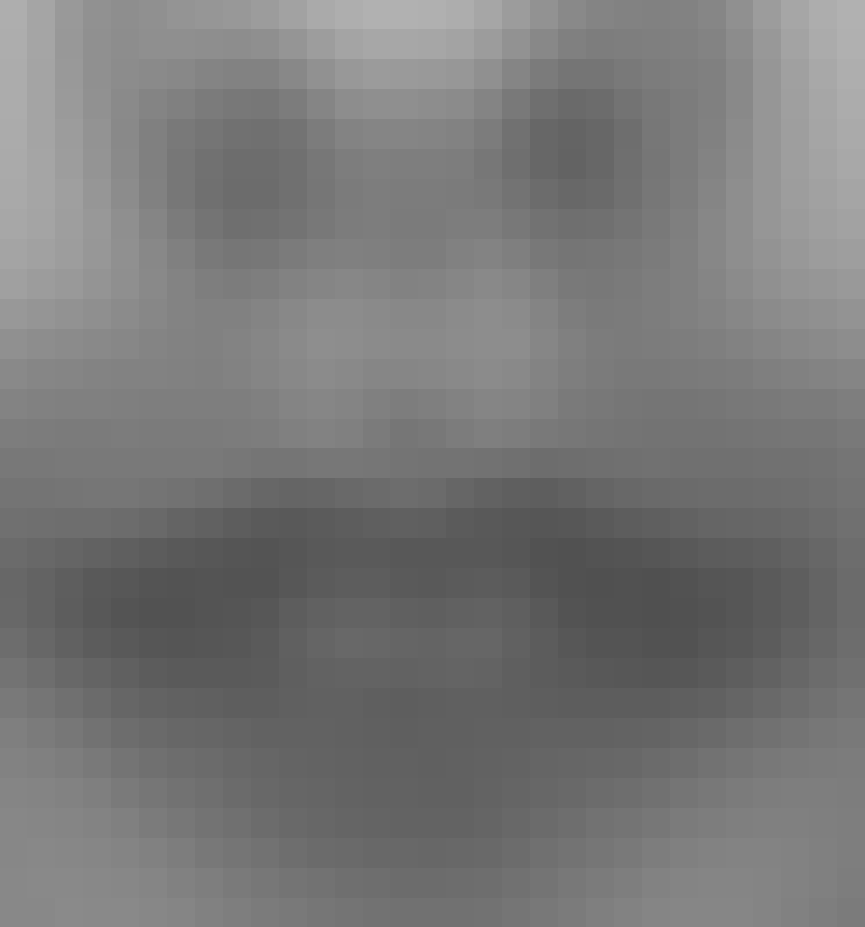
\includegraphics{figures/mouth_15.pdf}
\caption{Mean patch for mouth center top lip with `patch\_size = 15'}
\end{figure}

\section{Tensorflow\ldots{}}\label{tensorflow}

\section{Discussion and Comparison}\label{discussion-and-comparison}

\section{Conclusion}\label{conclusion}


\end{document}
